\documentclass{beamer}
\usepackage[utf8]{inputenc}
\usepackage[ngerman]{babel}
\usepackage{graphicx}
\usepackage{minted}
\usepackage[duration=25m,fontsize=28]{pdfpcnotes} % write Notes with \pnote{My custom note}
\usepackage{pgfgantt}
\usepackage{tikz}
\usepackage{pdfpc-commands}
\usetheme{kitovu}

\newcommand{\py}[1]{\mintinline{python}{#1}}

\title{Kitovu}
\subtitle{Engineering-Projekt FS 2018}
\author{Florian Bruhin \and Méline Sieber \and Nicolas Ganz}
\institute{HSR Hochschule für Technik Rapperswil}
\date{30. Mai 2018}

\begin{document}

  \maketitle
	
	\begin{frame}
	\frametitle{Das Problem: Skripte synchronisieren}
	% Ausgangsproblem: Files synchronisieren, schwierig, Florian Bruhin
	% Bisheriges: eigene Skripte (rsync), von Hand (mühsam), OpenHSR Connect (schwierig zum handhaben) - und: Moodle moosam Florian Bruhin
  \begin{columns}
    \column{0.55\linewidth}
    \begin{itemize}
      \item Herunterladen von Hand
      \item HSR Mapper \& ``alles ersetzen''
      \item OpenHSR connect
      \item Moodle Desktop
    \end{itemize}
    \column{0.4\linewidth}
    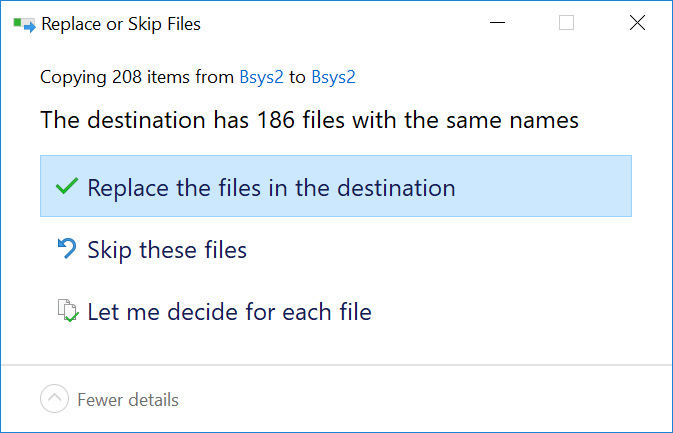
\includegraphics[width=\linewidth]{./img/windows_copy_dialog.png}
  \end{columns}
	\pnote{Frustrierendes Szenario, was viele {von euch, Studierende} kennen}
  \pnote{NEXT UP: Méline}
	\end{frame}
	
	\begin{frame}
	\frametitle{Unsere Lösung: Kitovu}
	\begin{center}
    \vspace{-1.7em}
		
\includegraphics[width=0.5\linewidth]{../../img/logo/kitovu.jpg}
	\end{center}
	\end{frame}

	\begin{frame}
		\frametitle{Unsere Lösung: Kitovu}
		\begin{center}
			
\includegraphics[width=0.5\linewidth]{./img/kitofu.png}
		\end{center}
		\pnote{-Logo aus Wortspiel entstanden...}
	\end{frame}

		\begin{frame}
			\frametitle{Unsere Lösung: Kitovu}
      \vspace{-0.8em}
			\begin{center}
				
\includegraphics[width=0.5\linewidth]{../../img/logo/kitovu.jpg} \\
				\textbf{Swahili: Knotenpunkt, Bauchnabel, "hub"}
			\end{center}
		\pnote{Swahili: Knotenpunkt, Bauchnabel, "hub"}
		\pnote{1 Client, 1 Knotenpunkt,  mit dem von verschiedenen Quellen Unterrichtsmaterialien synchronisiert werden können,
			das mit 1 Click}
		\pnote{Ziel: Studentinnen und Studenten der HSR möglichst einfach, möglichst ohne Aufwand 
			immer alle Materialien 
			auf dem eigenen Rechner haben,
			immer aktuellste Version}
		\end{frame}
	
	\begin{frame}
 	\frametitle{Wer benutzt kitovu?}
	 	\begin{columns}
%	 		\column[placement]{column width}
	 		\column{.2\textwidth}
	 		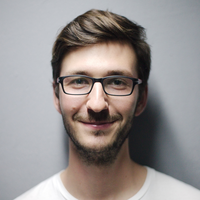
\includegraphics[width=0.9\linewidth]{./img/sven.png}
			\column{.8\textwidth}
			\textbf{Sven Färber, 20}
			\begin{itemize}
				\item Maturand
				\item Informatik, Vollzeit
				\item Windows-Nutzer (GUI)
			\end{itemize}
	 	\end{columns} \vspace{1em}
	 	\pause
		\begin{columns}
			%	 		\column[placement]{column width}
			\column{.2\textwidth}
			
\includegraphics[width=0.9\linewidth]{./img/leonie.png}
			\column{.8\textwidth}
			\textbf{Leonie Egger, 24}
			\begin{itemize}
				\item gelernte Floristin
				\item Informatik, Teilzeit
				\item erfahrene Arch-Linux-Nutzerin
			\end{itemize}
		\end{columns} \vspace{1em}
		\pause
		\begin{columns}
			\column{.2\textwidth}
			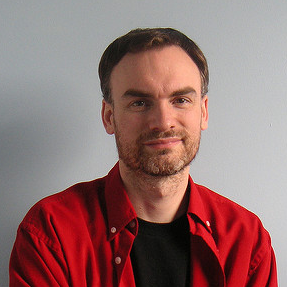
\includegraphics[width=0.9\linewidth]{./img/reto.png}
			\column{.8\textwidth}
			\textbf{Reto Schmid, 41}
		\begin{itemize}
			\item gelernter Grafiker, Vollzeitvater von drei Kindern
			\item Landschaftsarchitektur, Teilzeit
			\item Windows-Neuling, Mac-Nutzer
		\end{itemize}
		\end{columns}
		\pnote{FIKTIVE Persönlichkeiten ausgedacht}
		\pnote{Daraus: verschiedene Bedürfnisse abgeleitet}
		\pnote{* Leonie will Synchronisation automatisieren, selber mal kitovu erweitern}
		\pnote{* Sven: 1 Werkzeug für alle Plattformen}
		\pnote{* Reto: pendelt => zu Hause Unterrichtsmaterialien herunterladen, im Zug anschauen}
	\end{frame}
	
	\begin{frame}
	\frametitle{Kitovu im Kontext}
	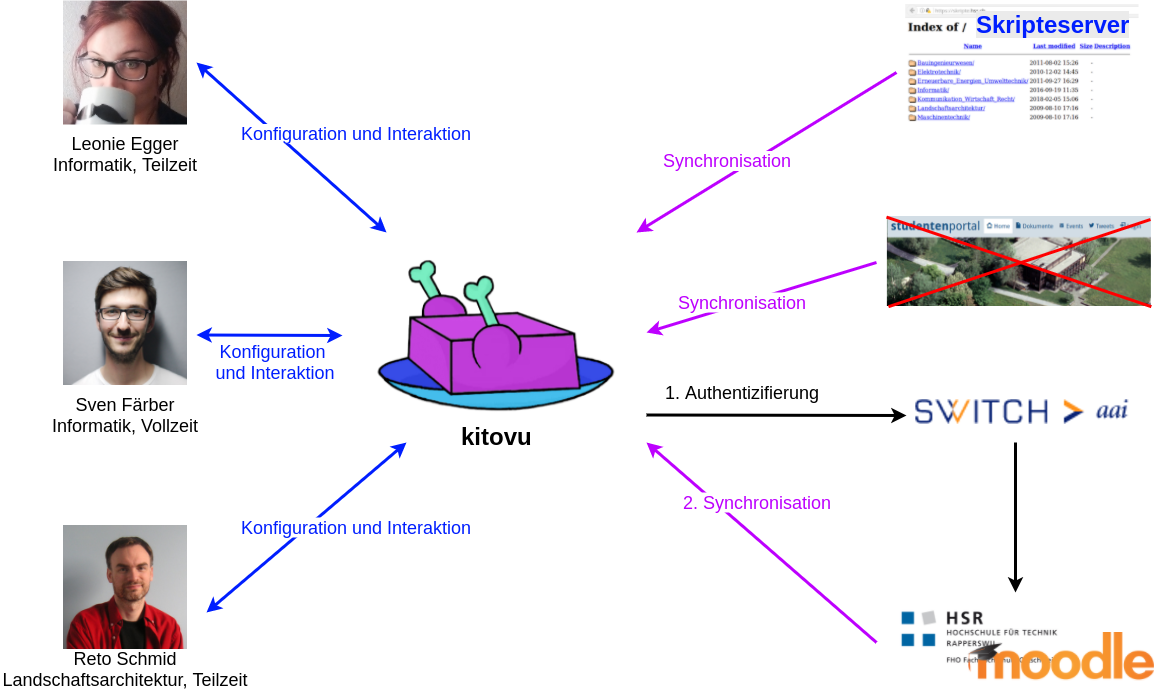
\includegraphics[width=\linewidth]{../03_End_of_Elaboration/img/kontextdiagramm.png}
	\pnote{* Knotenpunkt, Zentrum, um von verschiedenen Quellen Unterrichtsmaterialien herunterzuladen, möglichst wenig Aufwand}
	\pnote{*  Anfang Semester, einmal Konfiguration schreiben, was synchronisiert werden soll}
	\pnote{* dann Rest des Semesters: 1 klick pro Woche, pro Tag und neue Unterrichtsmaterialien werden auf den eigenen Laptop heruntergeladen}
	\pnote{* gehen später darauf ein, weshalb Studentenportal durchgestrichen.}
	\pnote{NEXT UP: Nicolas}
	\end{frame}

  \begin{frame}
    \frametitle{Demo}
    \vspace{-0.5em}
    \begin{center}
      % Additional options: loop
      \inlineMovie[autostart&start=4]{img/demo.mp4}{img/blank.png}{width=0.85\linewidth, height=0.6375\linewidth}
    \end{center}

    \pnote{- CMD: Einmal Sync ohne Daten -> langsam}
    \pnote{- CMD: Zweiter Sync -> schnell & weniger Output}
    \pnote{- GUI: Zeigen, dass es den selben Output hat}
    \pnote{NEXT UP: Méline}
  \end{frame}

	\begin{frame}
		\frametitle{Projektumfang}
		\begin{itemize}
			\item Ablauf der Software-Entwicklung kennenlernen
			\item Kleines Projekt, aber ausbaubar
			\begin{itemize}
				\item \emph{kitovu}-Code: 1'177 Zeilen
				\item Test-Code: 1'405 Zeilen
			\end{itemize}
			\item Skripteserver: muss funktionieren
			\begin{itemize}
				\item Optional: Moodle, Studentenportal
			\end{itemize}
			\item Kommandozeile: muss funktionieren
			\begin{itemize}
				\item Optional: grafische Benutzeroberfläche (rudimentär)
			\end{itemize}
		\end{itemize}
	\pnote{* Fokus darauf, Ablauf der Software-Entwicklung kennenlernen}
	\pnote{* Nur zu dritt: klein, aber ausbaubar => handvoll Klassen, rund 1000 Zeilen Code, gleich viel Test-Code}
	\pnote{* Kernziel: Skripteserver anbinden, optional definiert: Moodle, Studentenportal}
	\pnote{* Kommandoziele muss funktionieren, optional: grafische Benutzeroberfläche}
	\pnote{=> Herangehensweise gelohnt => sehen wir beim Projekt-Fazit}
	\pnote{* Zeit: Nicolas, ich: arbeiten beide, Florian: Vollzeitstudent }
	\pnote{=> nicht so flexibel, kluge Zeitplanung ein Muss}
	\end{frame}
	
	\begin{frame}
		\frametitle{Zeitplan}
		\vspace{-1em}
		\begin{center}
			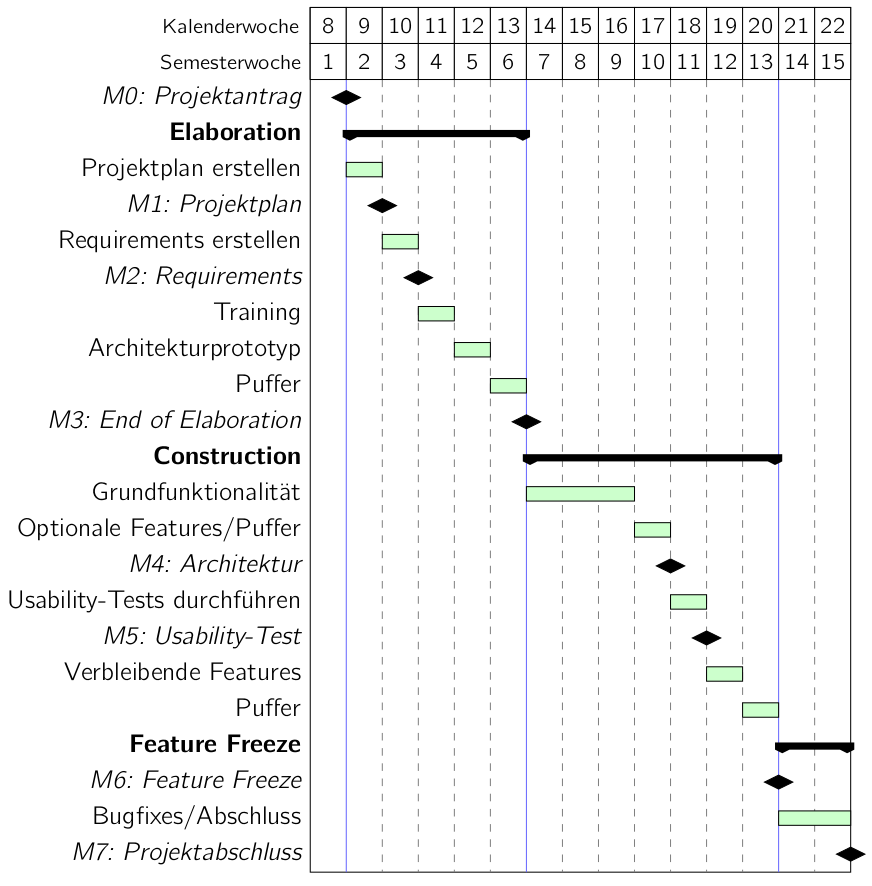
\includegraphics[height=0.9\textheight]{./img/zeitplan.png}
		\end{center}
		\pnote{* extra Trainingsphase => gelohnt}
		\pnote{* End of Elaboration: erster Prototyp, da klar, welche Plattformen funktionieren werden}
		\pnote{* Flo war nach Ostern 2 Wochen krank, grad Beginn Construction-Phase}
		\pnote{=>, trotzdem geklappt und vorangekommen}
		\pnote{* Architektur um 1 Woche verschoben, damit auch Usability-Tests}
		\pnote{NEXT UP: Nicolas}
	\end{frame}
	
	\begin{frame}
	\frametitle{Plattformunabhängigkeit}
	
	% Plattformunabhängigkeit: Dahinterliegende Technologie: Python, was ist SMB, PySMB Nicolas Ganz
	\begin{itemize}
	  \item[]
	    
\includegraphics[height=1.5em]{./img/python-logo-small.png}
	    \begin{itemize}
	      \item Konzeptionell plattformunabhängig
	      \item Unterstützung bei Pfad-Definitionen
	    \end{itemize}
      \vspace{1em}
	  \item[]
	    
\includegraphics[height=1.5em]{./img/Qt-logo.png}
	    \begin{itemize}
	      \item Framework für GUIs
	      \item Verwendet mit \emph{PyQt}
	    \end{itemize}
	\end{itemize}
	\end{frame}

  \begin{frame}
    \frametitle{Plattformunabhängigkeit - Externe Schnittstellen}

    \begin{itemize}
      \item Moodle
        \begin{itemize}
          \item REST-ähnlich
          \item Angebunden mit \emph{requests}
        \end{itemize}
      \item Skripteserver
        \begin{itemize}
          \item SMB - Server Message Block
          \item Windows-Netzwerkordner
          \item Angebunden mit \emph{PySMB}
        \end{itemize}
    \end{itemize}
    \pnote{NEXT UP: Florian}
  \end{frame}

	\begin{frame}
	\frametitle{Kitovu ist erweiterbar}
	% Kontextdiagramm: Erweiterbarkeit wichtig => Plugin-Architektur Florian Bruhin
	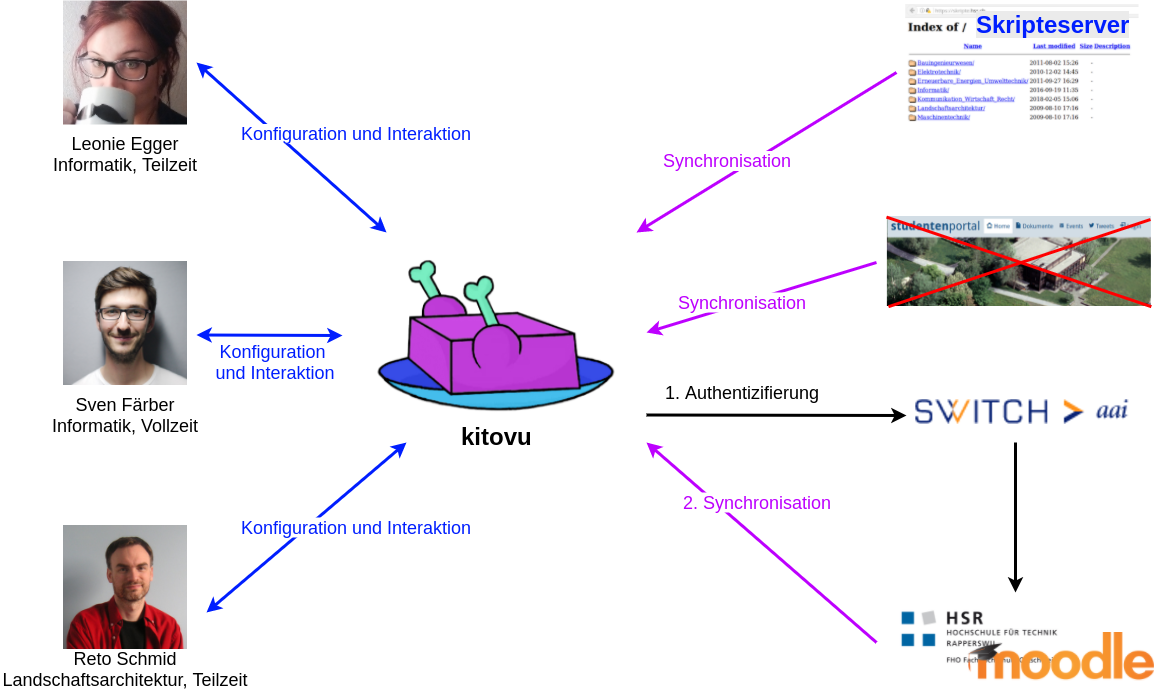
\includegraphics[width=\linewidth]{../03_End_of_Elaboration/img/kontextdiagramm.png}
	\end{frame}
	
	\begin{frame}[fragile]
	\frametitle{Kitovu ist erweiterbar}

  \begin{itemize}
    \item \py{configure(self, info: Dict[str, Any]) -> None}
    \item \py{connect(self) -> None}
    \item \py{list_path(self, path: PurePath) -> Iterable[PurePath]}
    \item \py{create_local_digest(self, path: Path) -> str}
    \item \py{create_remote_digest(self, path: PurePath) -> str}
    \item \py{retrieve_file(self, path: PurePath,} \\ \hspace{7em} \py{fileobj: IO[bytes]) -> Optional[int]}
    \item \py{disconnect(self) -> None}
  \end{itemize}
  	\pnote{NEXT UP: Nicolas}
\end{frame}

  \begin{frame}
    \frametitle{Unser Workflow - JIRA \& Confluence}
    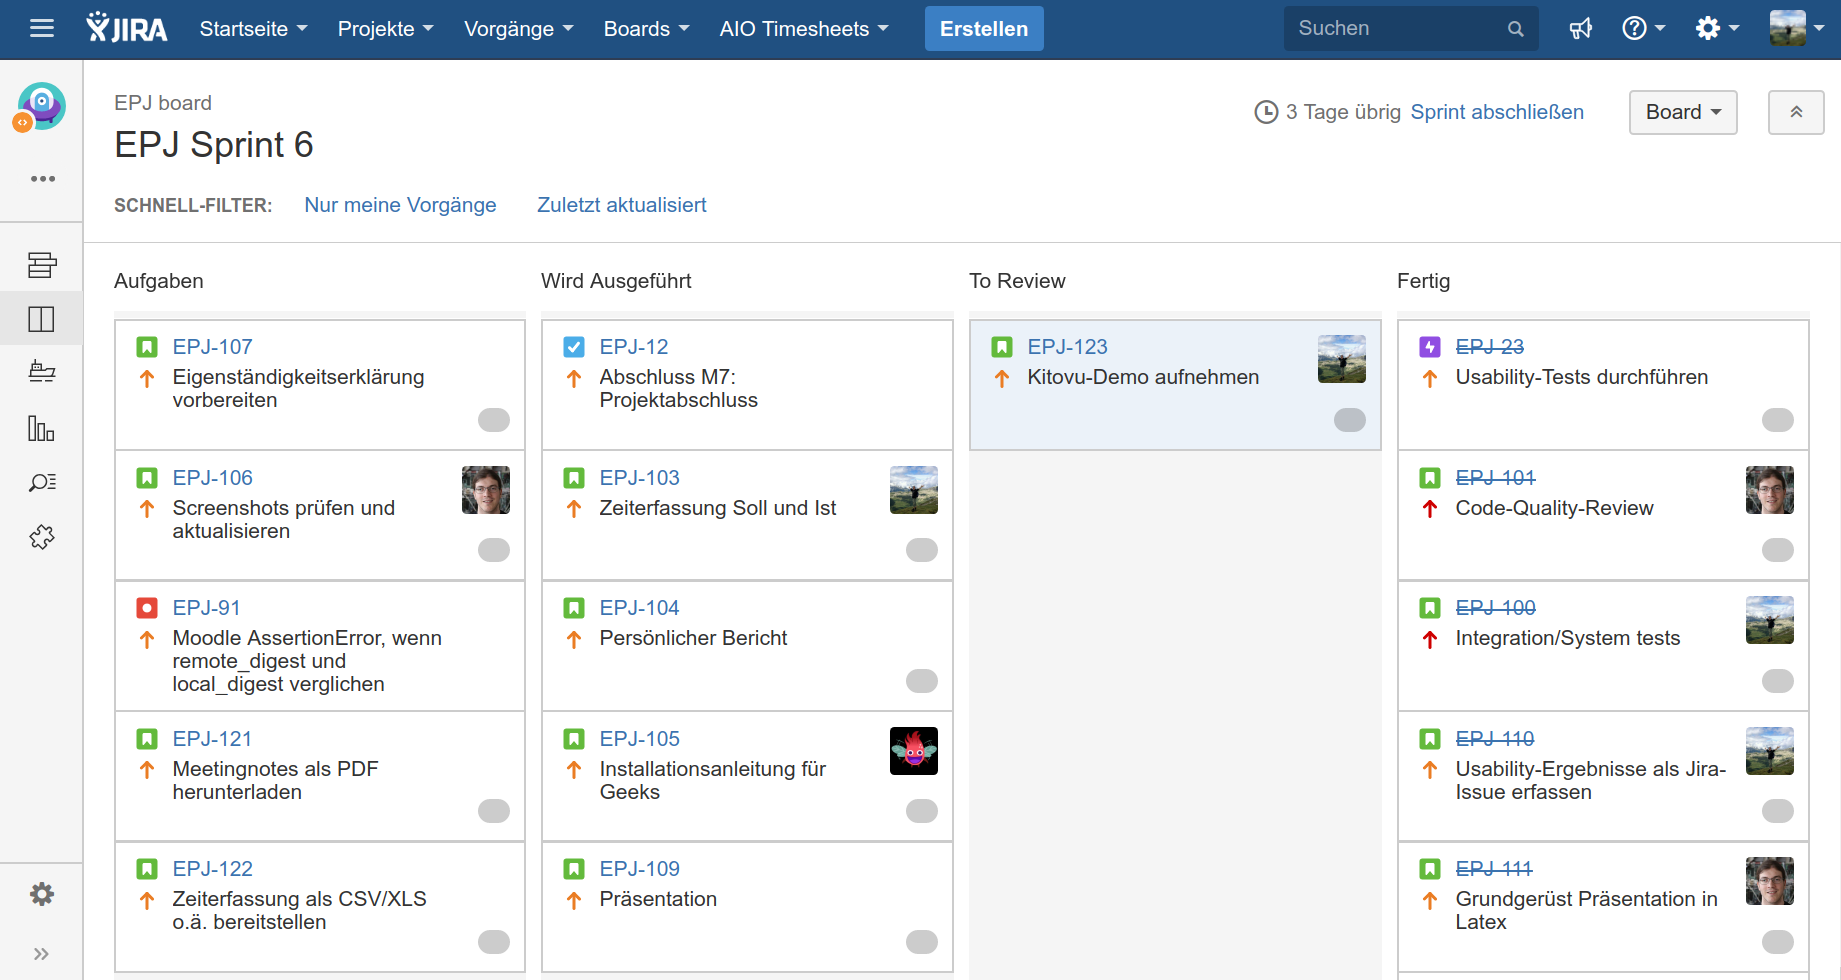
\includegraphics[width=\linewidth]{./img/jira_board.png}
    \pnote{NEXT UP: Florian}
  \end{frame}

	\begin{frame}
	\frametitle{Unser Workflow - GitHub \& Codecov}
  \begin{center}
	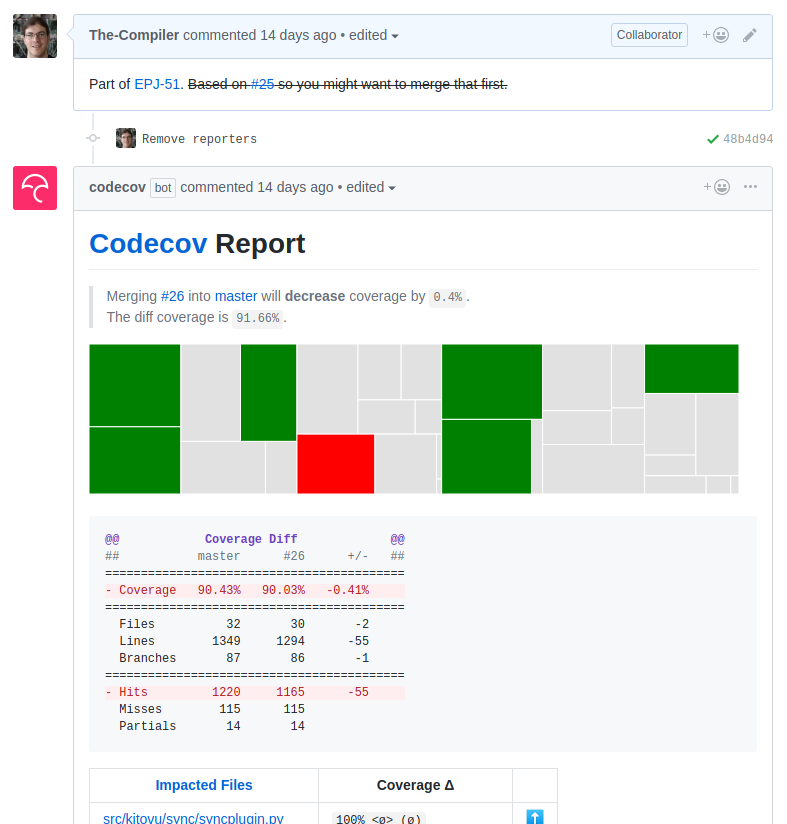
\includegraphics[height=0.8\textheight]{img/github.png}
  \end{center}
	\pnote{GitHub und Opensource - Bots, Tests/Coverage}
	\end{frame}

	\begin{frame}
	\frametitle{Unser Workflow - Travis \& AppVeyor}
	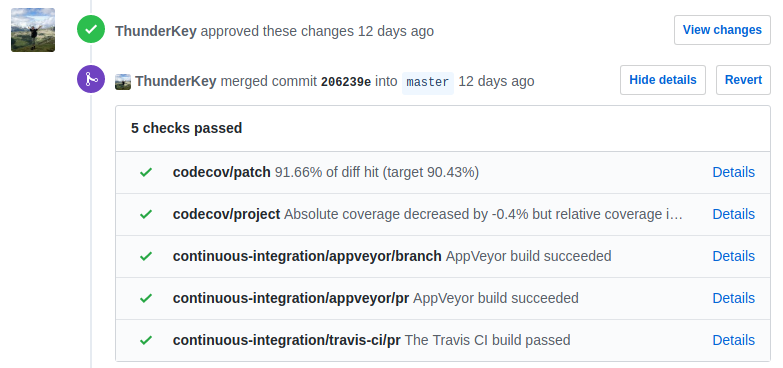
\includegraphics[width=\linewidth]{img/github-checks.png}
	\end{frame}

	\begin{frame}[fragile]
	\frametitle{Unser Workflow - pytest}
  \begin{verbatim}
tests/test_cli.py ............                     [  9%]
tests/test_dummyplugin.py .........                [ 16%]
tests/test_filecache.py ..............             [ 27%]
tests/test_utils.py .........                      [ 34%]
tests/gui/test_confscreen.py .....                 [ 37%]
tests/gui/test_mainwindow.py ...                   [ 40%]
tests/gui/test_startscreen.py ...                  [ 42%]
tests/gui/test_syncscreen.py .......               [ 48%]
tests/sync/test_moodle.py ........................ [ 66%]
tests/sync/test_settings.py .....                  [ 70%]
tests/sync/test_smb.py ....................        [ 86%]
tests/sync/test_syncing.py ..................      [100%]

============== 129 passed in 2.48 seconds ==============
  \end{verbatim}
\end{frame}

  \begin{frame}[fragile]
    \frametitle{Unser Workflow - mypy}

    % https://github.com/gpoore/minted/issues/70#issuecomment-111729930
    \begingroup
    \catcode`\!=\active
    \def!#1!{\colorbox{yellow}{#1}}
    \begin{minted}[escapeinside=||]{python}
def retrieve_file(self, path: |!PurePath!|,
                  fileobj: |!IO[bytes]!|) -> |!Optional[int]!|:
    moodle_file: |!MoodleFile!| = self._files[path]
    # [...]
    \end{minted}
    \endgroup
   	\pnote{NEXT UP: Méline}
\end{frame}
	
	\begin{frame}
	\frametitle{Fazit und Erfahrungen}
\begin{center}
	
\includegraphics[width=20 em]{./img/unicorn.png}
	\end{center}
	\pnote{voller positiven Überraschungen, wie Einhorn, weil so selten}
	\end{frame}
	
	\begin{frame}
    % Fazit & Erfahrungen (3 Erfahungsberichte) Méline Sieber Gesamt: Moodle war grösste Überraschung, Studentenportal grösste Enttäuschung. Allergrösste Überraschung: alles reibungslos <3, Pair Programming super nützlich, Code Reviews, persönliche Kommunikation total wichtig (Meetings)
		\frametitle{Fazit und Erfahrungen}
		\begin{columns}
				\column{.45\textwidth}
			Alle Ziele erreicht
				\begin{itemize}
					    \item Grösste Überraschung: Moodle
					    \item Grösste Enttäuschung: Studentenportal
				\end{itemize}
			Sehr gute Teamdynamik
			\begin{itemize}
				\item Wochen-Meetings	
				\item Pair-Programming
			\end{itemize}
			Code-Style-Regeln, strenge Code-Reviews
			\column{.45\textwidth}
			
\includegraphics[width=0.9\linewidth]{./img/unicorn.png}
		\end{columns}
		\pnote{* Alle Ziele erreicht! Grösste Überraschung: Moodle; Grösste Enttäuschung: Studentenportal}
		\pnote{* Gute Teamdynamik:}
		\pnote{=> Wöchentliche Besprechungen, Entscheidungen von allen getragen}
		\pnote{=> Pair-Programming => zeigt sich in Zeiterfassung Soll/Ist, weil Zeit doppelt}
		\pnote{=> Code-Style-Regeln gesetzt, strenge Code-Reviews}
		\pnote{NEXT UP: Nicolas}
	\end{frame}

  \begin{frame}
    \frametitle{Fazit: Zeiterfassung}
    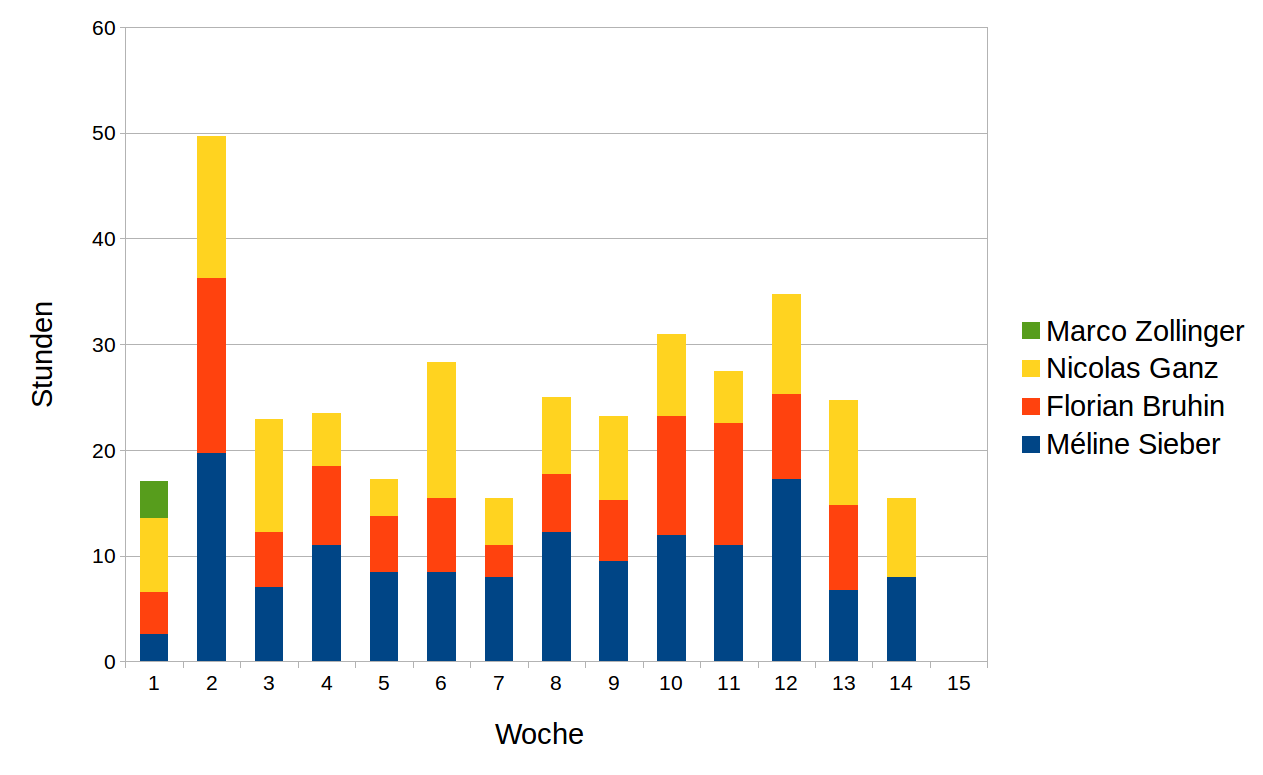
\includegraphics[width=\linewidth]{./img/time_per_person.png}
    \pnote{NEXT UP: Méline}
  \end{frame}

  \begin{frame}
    \frametitle{Fazit: Zeitschätzungen}
    \includegraphics[width=\linewidth]{./img/time_per_issue.png}
    \pnote{NEXT UP: Méline}
  \end{frame}

	\begin{frame}
	  	\frametitle{Persönliche Erfahrungen: Méline Sieber}
	  	Ausgangslage: 
		\begin{itemize}
			\item Wenig Programmiererfahrung, etwas Python-Skripting
			\item Quereinsteigerin
		\end{itemize}
		\pause
		Projektende:
			\begin{itemize}
				\item Pair-Programming unverzichtbar
				\item Team-Chemie stimmt, Wochenmeetings
				\item Programmierroutine: Ziel erreicht
				\item Riesenspass :)
			\end{itemize}
		\pnote{* Wasser war sehr kalt => mehr schwimmen => wärmer}
		\pnote{* Wenig Programmiererfahrung}
		\pnote{=> Pair-Programming: sehr viel gelernt, Probleme zusammen gelöst => danke}
		\pnote{=> meine grösseren Problem => Knacknüsse des Projekts}
		\pnote{* Wochenmeetings enorm wichtig, gemerkt, wann wir nicht vom gleichen sprachen, aufeinander Vision abstimmen}
		\pnote{* Ziel: Programmierroutine erreicht}
		\pnote{FUUUUN}
		\pnote{NEXT UP: Florian}
	\end{frame}
	
	\begin{frame}
	   	\frametitle{Persönliche Erfahrungen: Florian Bruhin}
      \begin{itemize}
        \item Viele ``soziale'' Dinge, aber auch technische.
        \item Geniales Team!
        \item Es ist so viel wert, sich regelmässig zu sehen!
        \item ``End of elaboration'' ist keine schlechte Idee
      \end{itemize}
	\end{frame}

  \begin{frame}
    \frametitle{Persönliche Erfahrungen: Nicolas Ganz}

    Umstellung zu Python:
    \begin{itemize}
      \item Aus Ruby
      \item Harte Guidelines
    \end{itemize}

    \pause
    Kommunikation im Team:
    \begin{itemize}
      \item Konstruktive Diskussionen
      \item Gründliche Code-Reviews
    \end{itemize}

    \pause
    Projektidee:
    \begin{itemize}
      \item Motiviert
      \item Studiengangübergreifendes Interesse
    \end{itemize}
  \end{frame}

  \begin{frame}
  \frametitle{Kitovu lebt weiter}
  % Ausblick: schönere GUI machen => Usability hat das gezeigt, Release für HSR-Studis, Sommerprojekt Nicolas Ganz

  Grössere offene Punkte:
  \begin{itemize}
    \item GUI verbessern
    \item Konfliktbehandlung
  \end{itemize}

  Entwicklung:
  \begin{itemize}
    \item Sommerprojekt
    \item Ziel: Nächstes Semester einsatzbereit
  \end{itemize}
  \end{frame}

  \begin{frame}
  \frametitle{Kontakt}
  \begin{columns}
    \column{0.45\linewidth}
    \begin{itemize}
      \item Florian Bruhin \\ \url{florian.bruhin@hsr.ch} \\[2em]
      \item Méline Sieber \\ \url{meline.sieber@hsr.ch} \\[2em]
      \item Nicolas Ganz \\ \url{nicolas.ganz@hsr.ch}
    \end{itemize}

    \column{0.5\linewidth}
		
\includegraphics[width=\linewidth]{../../img/logo/kitovu.jpg}
  \end{columns}
  \end{frame}
\end{document}
